\section{Firmware Design and Implementation}

This section describes the firmware developed for the STM32U5 microcontroller~\cite{stm32u5}, which forms the core of our low-energy backup communication system. It handles real-time LoRa communication, sensor data acquisition, and voice output via speech synthesis or WAV playback. To guarantee deterministic timing, we build on FreeRTOS~\cite{freertos}, as illustrated in Figure~\ref{fig:firmware-system}. Task isolation and priority levels make the codebase modular and maintainable.

\begin{figure}[H]
\centering
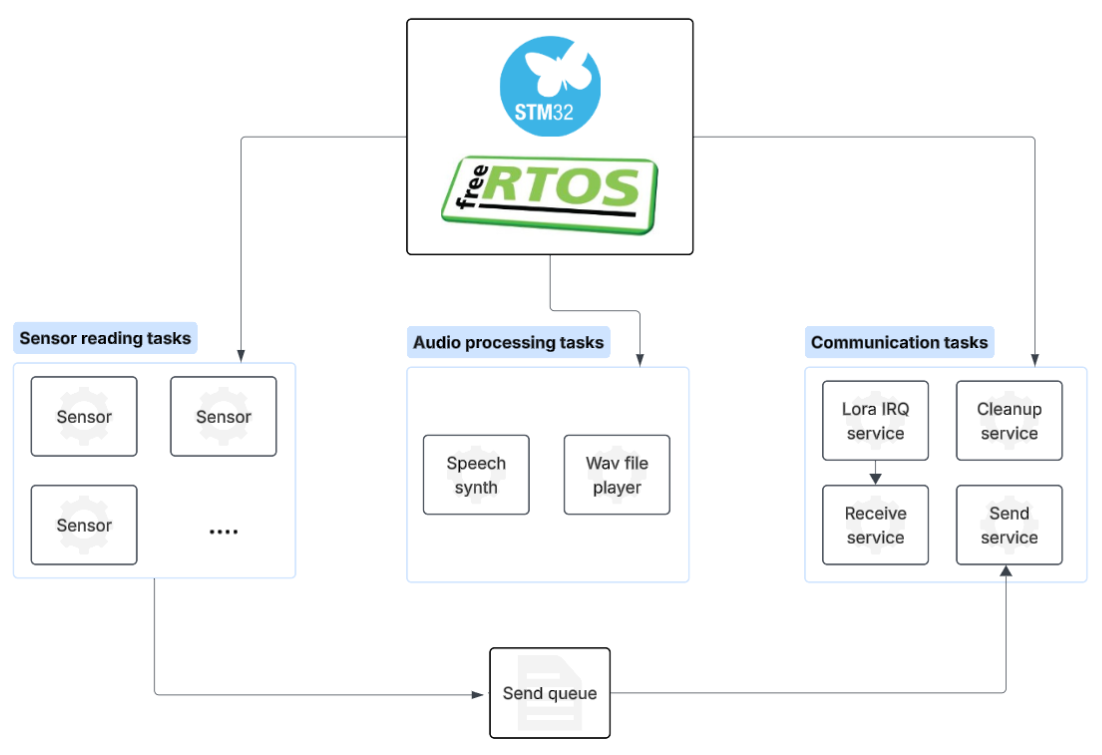
\includegraphics[width=0.45\textwidth]{images/firmware-system-design.png}
\caption{Overview of the FreeRTOS-based firmware architecture}\label{fig:firmware-system}
\end{figure}

\subsection{Overall Architecture}

Figure~\ref{fig:firmware-system} shows three primary functional domains, each implemented as one or more FreeRTOS tasks communicating via inter-task communication mechanisms provided by FreeRTOS.

\subsection{LoRa Communication}
\begin{itemize}
  \item \textbf{IRQ Handler}
    Waits on the SX1276~\cite{sx1276} interrupt line to detect packet RX/TX completion, then gives a binary semaphore.
  \item \textbf{Receive Task}
    Blocks on that semaphore, retrieves incoming packets, decrypts them with hardware-accelerated AES-128 in CTR mode, and forwards them for processing.  
  \item \textbf{Transmit Task}
    Pulls outgoing messages from a FreeRTOS queue, encrypts and formats them, then issues the LoRa send command.
  \item \textbf{Cleanup Task}
    Periodically scans stored packet buffers for timeouts and frees associated heap memory.
\end{itemize}

The message formatting steps mentioned above, including encryption, fragmentation, and encapsulation, are detailed in Section~\ref{sec:message-processing}.

\subsection{Sensor Management}
Each sensor (e.g.\ temperature, pressure, speed) runs its own task at a low priority. Tasks periodically sample the hardware interface, package readings, and enqueue them for transmission.

\subsection{Audio Processing}
\begin{itemize}
  \item \textbf{Speech Synthesis Task}
    A port of \texttt{espeak-ng}~\cite{espeakng} with all file I/O replaced by in-memory C arrays. Which dequeues strings from a FreeRTOS queue, synthesises, streams audio to I2S hardware.
  \item \textbf{WAV playback Task}
    Streams hard-coded WAV data (e.g.\ racing flags, standard phrases) to the I2S hardware.
\end{itemize}

\subsection{Power and Memory Management}

All tasks are assigned carefully chosen priorities (Table~\ref{tab:priorities}) so that time-critical communication tasks preempt lower-priority work. We enable FreeRTOS tickless idle to allow the STM32U5 to enter deep sleep whenever the system is idle.

\begin{table}[H]
  \centering
  \caption{Task priorities and stack usage}
  \label{tab:priorities}
  \begin{tabular}{lrr}
    \hline
    Task                     & Priority & Stack (bytes) \\
    \hline
    LoRa IRQ Handler         & 8        & 128            \\
    Speech Synthesis         & 7        & 48\,000        \\
    WAV Playback             & 7        & 256            \\
    LoRa Transmit            & 5        & 128            \\
    Cleanup                  & 5        & 128            \\
    Sensor (each)            & 3        & 256            \\
    \hline
  \end{tabular}
\end{table}

\subsection{Fragmentation and Reassembly of Encrypted Messages}\label{sec:message-processing}

The transmission process, illustrated in Figure~\ref{fig:fragmentation-flow}, begins with raw message data assigned a unique ID. This data is then processed through the following steps:

\textbf{Message Transmission Pipeline}
\begin{enumerate}
  \item The raw message is padded using PKCS\#7 to ensure its length is a multiple of 16 bytes, satisfying the requirements of the hardware-acelerated AES module.
  \item The padded message is encrypted using AES-128 in CTR mode.
  \item The resulting ciphertext is fragmented into fixed-size chunks. Each fragment is encapsulated in a packet containing the meassage ID, fragment index, and total number of fragments.
  \item Packets are enqueued for transmission via LoRa.
\end{enumerate}

\textbf{Message Reception Pipeline}
\begin{enumerate}
  \setcounter{enumi}{4}
  \item Recieved packets are collected in a queue.
  \item Each packet is decapsulated and sorted by message ID. Once all fragments of a message are received, they are reassembled into the full encrypted message.
  \item The complete ciphertext is decrypted to recover the padded plaintext.
  \item Padding is removed, restoring the original raw message.
\end{enumerate}

\begin{figure}[H]
  \centering
  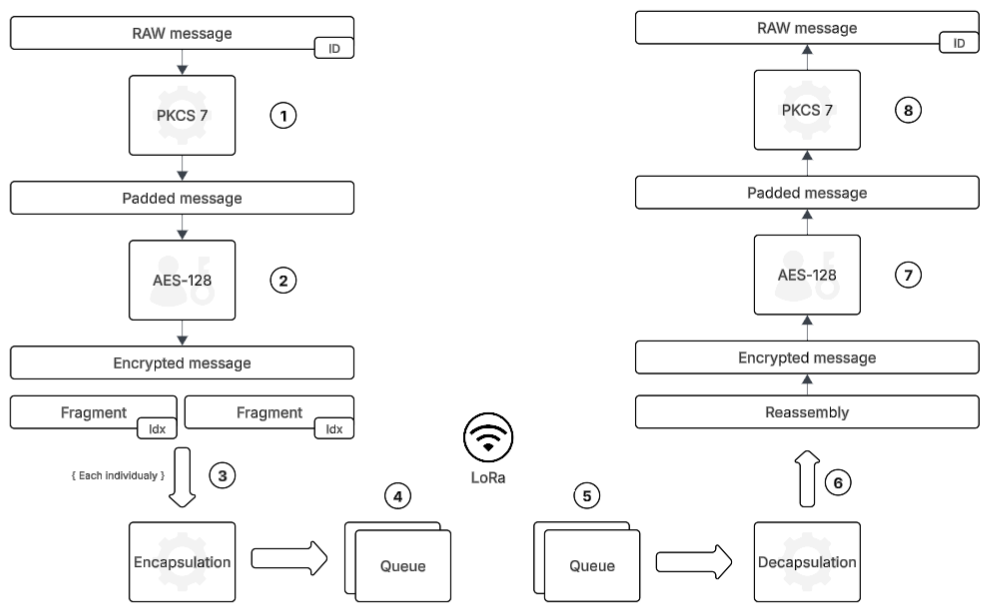
\includegraphics[width=0.45\textwidth]{images/packet-fragmentation-flow.png}
  \caption{Flowchart illustrating the message encryption fragmentation process prior to LoRa transmission.}
  \label{fig:fragmentation-flow}
\end{figure}

